\subsection{Concept }
We propose a canvas system wherein the user may drag e-learning modules from a 
toolbox, and drop them onto the canvas, as in Figure~\ref{fig:adding}. The 
modules may be empty or finished. If they are empty, then the authoring tool 
for said module opens. If it is not empty, then the user may further edit it 
if they wish. In addition to drag-and-drop, the user may also use an ``add'' 
button, as drag-and-drop is not viable for universal design.

\begin{figure}[H]
    \centering
    \begin{scale}{0.1}
        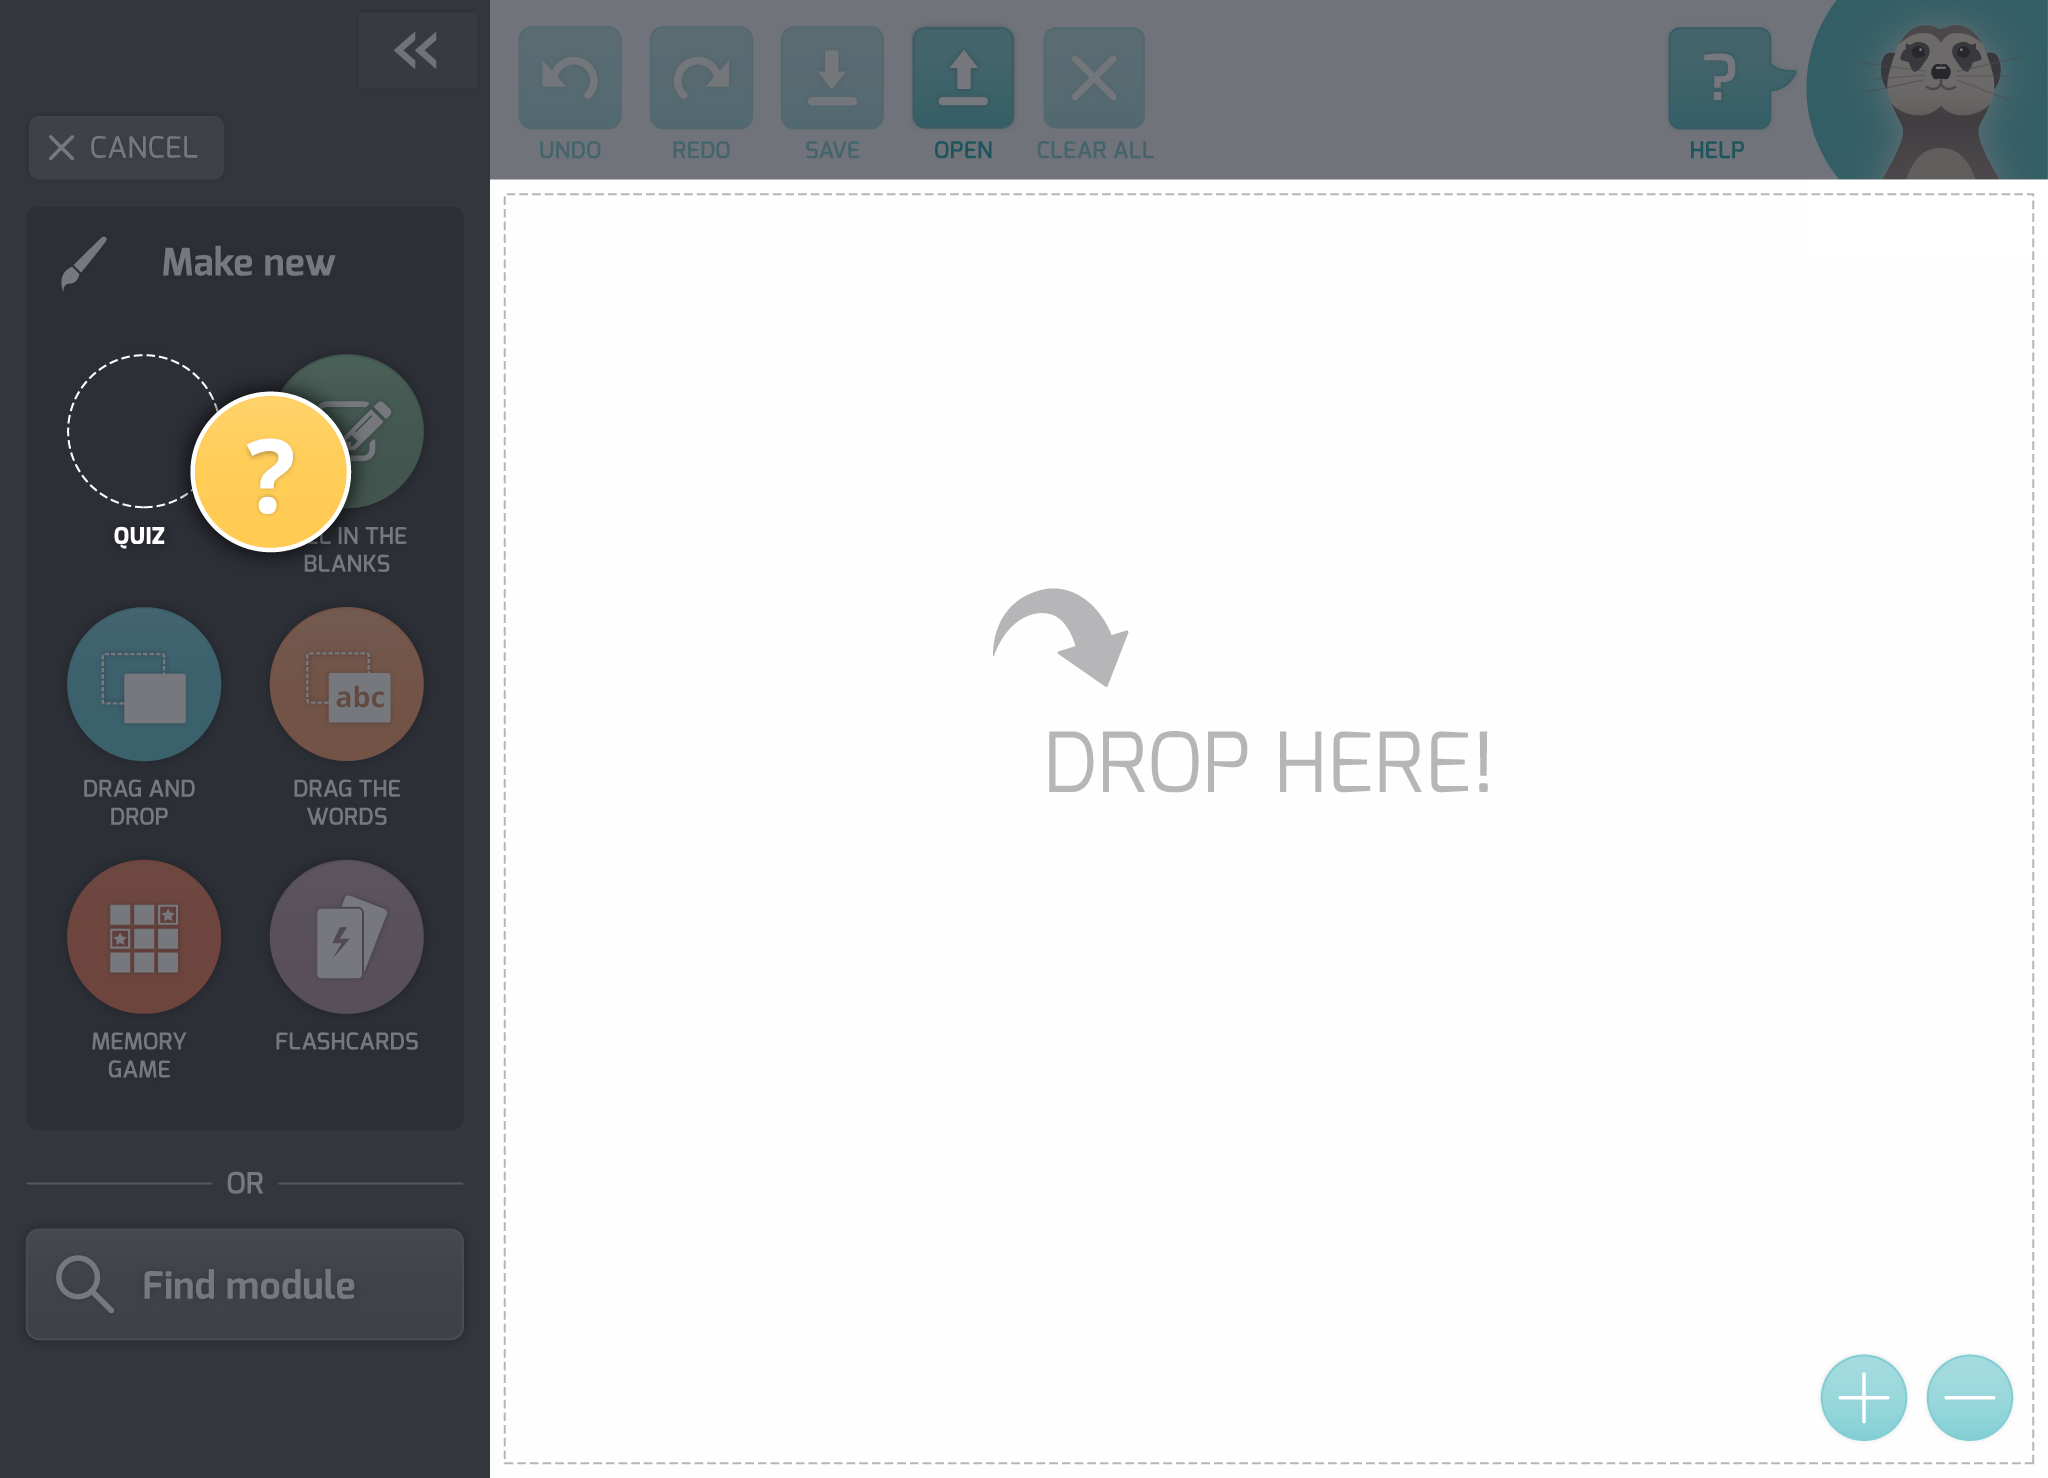
\includegraphics{fig/adding.png}
    \end{scale}
    \caption{A user dragging a module onto the canvas to add it}
   \label{fig:adding}
\end{figure}

To schedule data and control flow, the user drags arrows between the modules 
on the canvas. These associations may be customised. ``If the user finished 
[module a] with a score of more than 80\% correct, then direct them to [module 
b]; if the user did not, then direct them to [module c]''. A simple 
illustration of this is in Figure~\ref{fig:arrows}.

\begin{figure}[H]
    \centering
    \begin{scale}{0.1}
        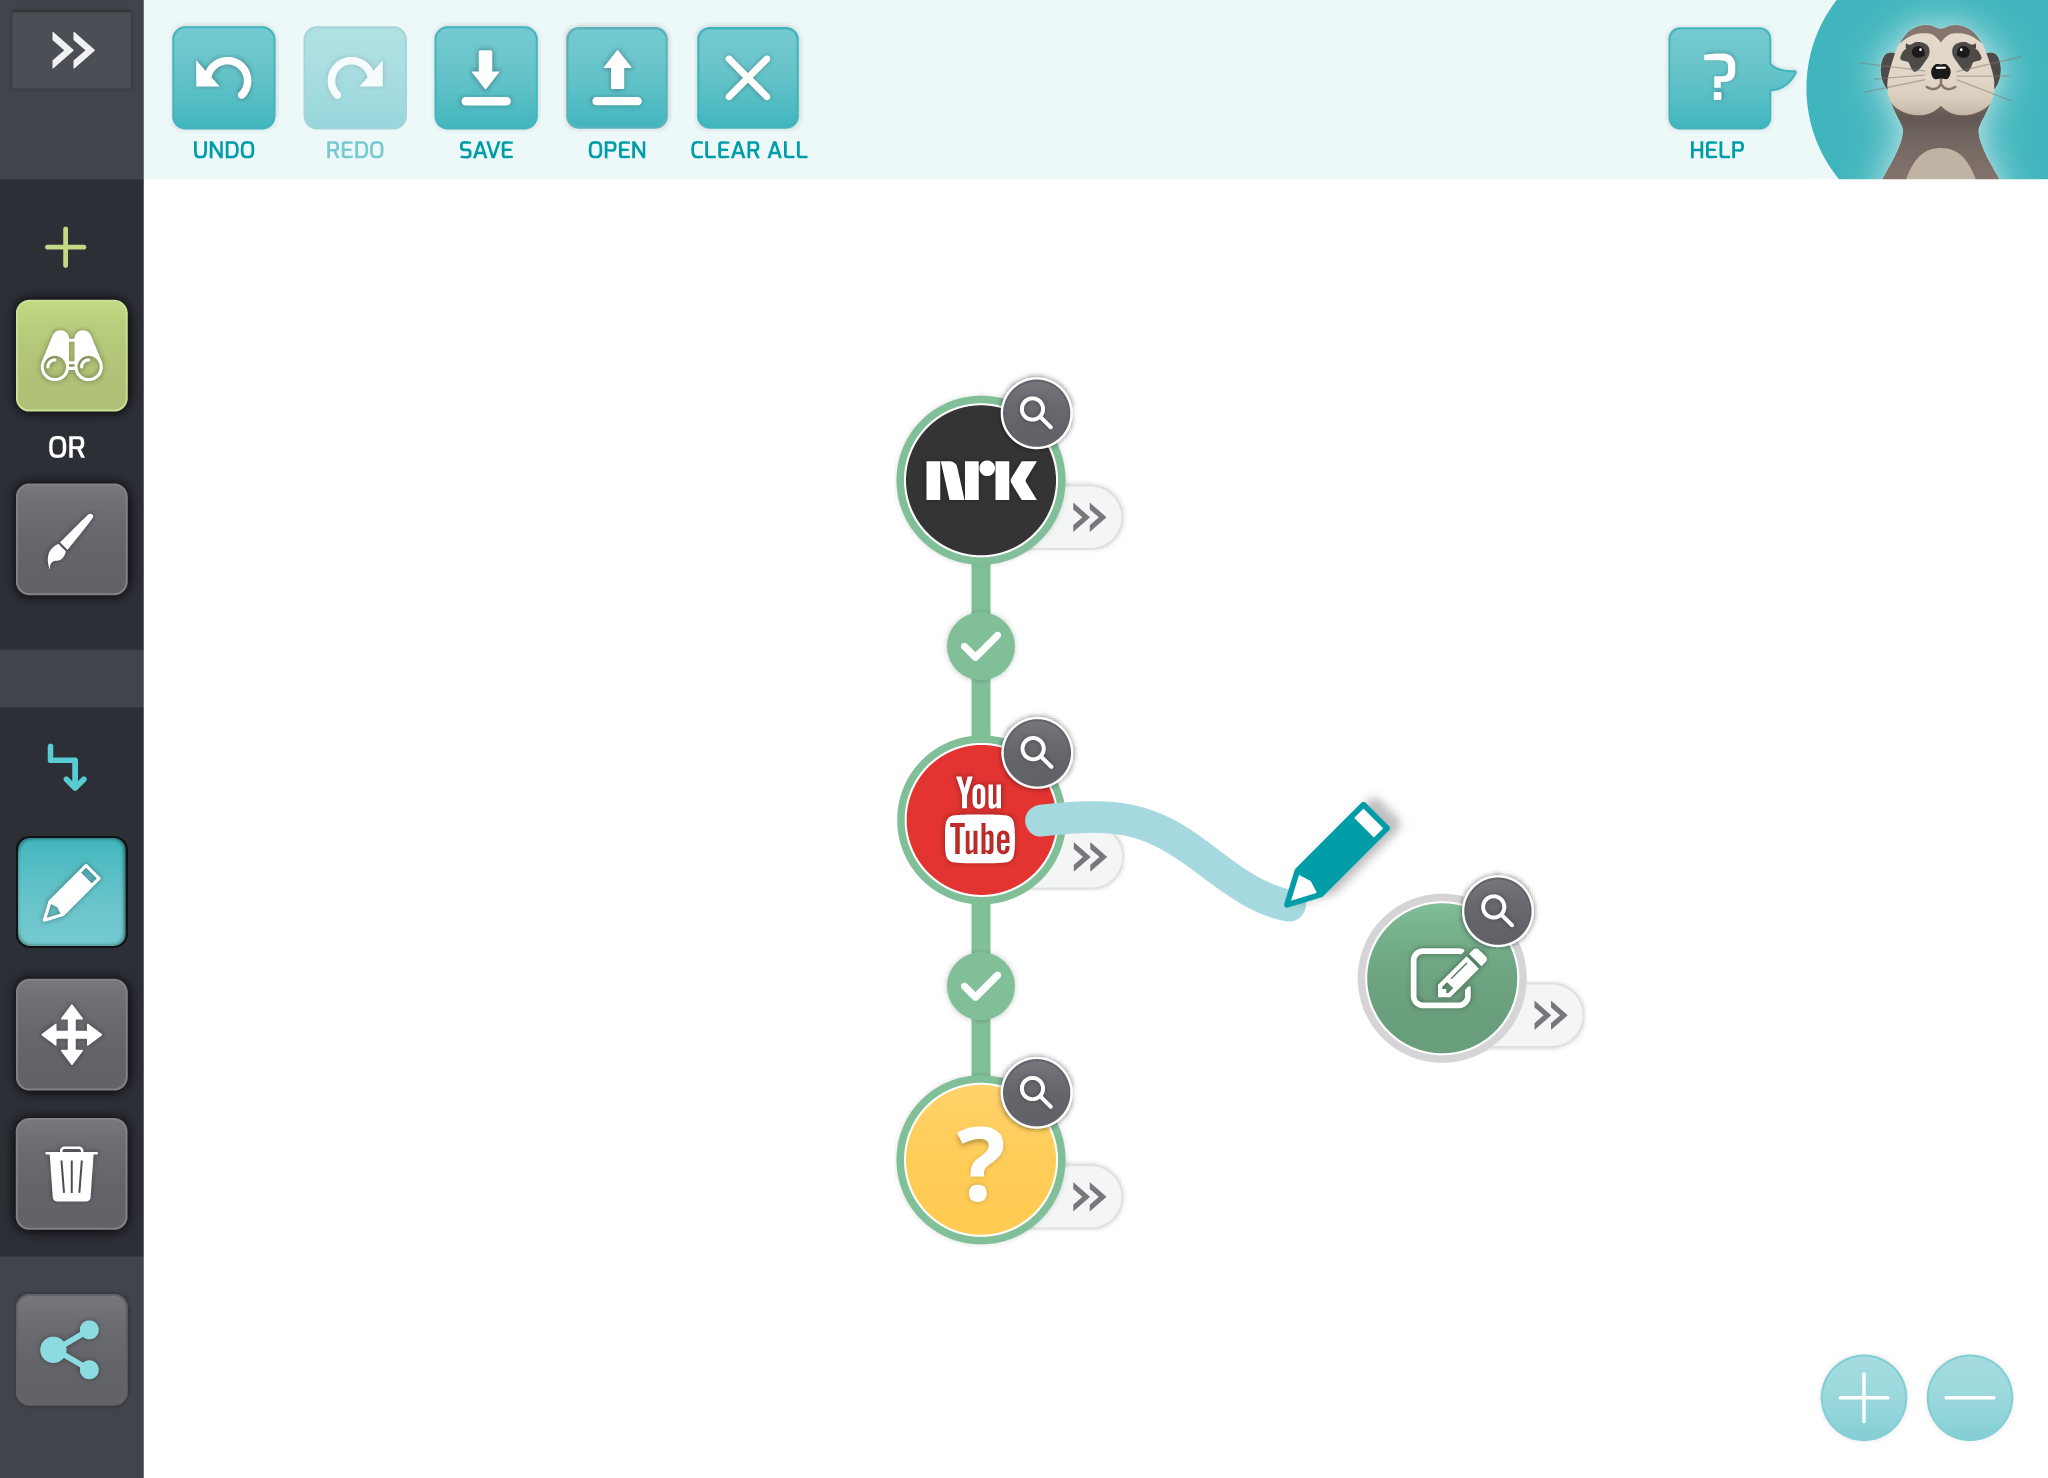
\includegraphics{fig/arrows.png}
    \end{scale}
    \caption{Visualised control flow}
   \label{fig:arrows}
\end{figure}

Compositions are modules themselves.

When a user wants to compose modules, users may search for which modules to 
use. We want to encourage reuse and remixing rather than novelties. 
Consequently we focus the search option before the ``author new module'' 
option. The search option is shown in Figure~\ref{fig:search}, which also 
shows results filtering in action.

\begin{figure}[H]
    \centering
    \begin{scale}{0.1}
        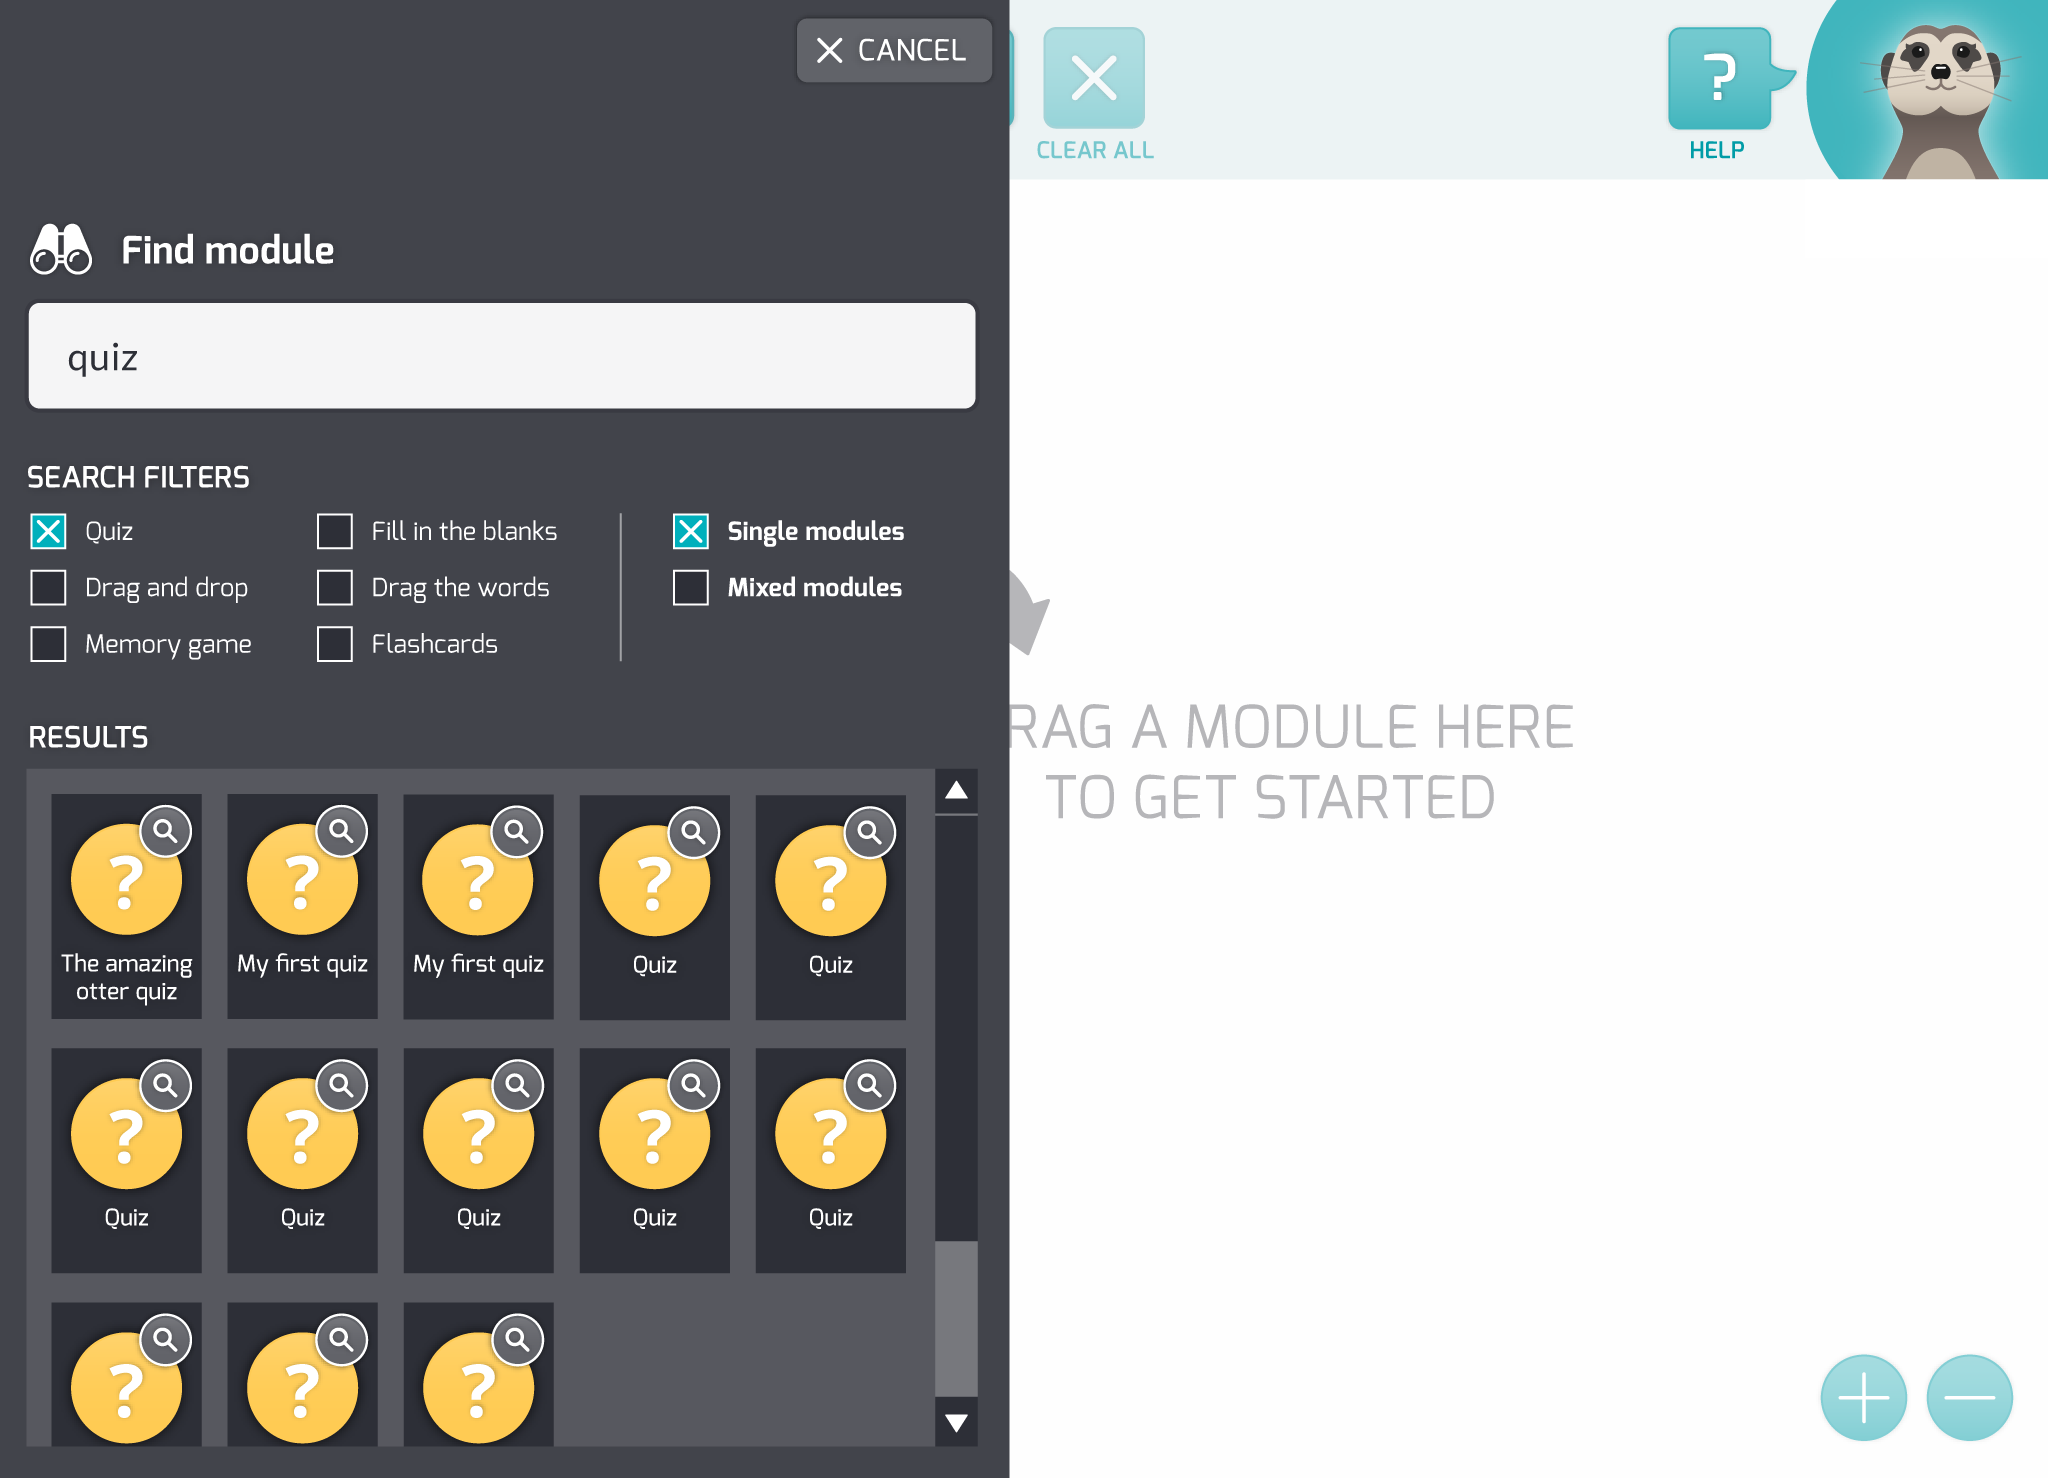
\includegraphics{fig/search.png}
    \end{scale}
    \caption{Search results, filtered by type}
   \label{fig:search}
\end{figure}

As another incentive, when a user authors a new module, we track reuses and 
remixes. Users may in a presentation of all their authored modules see how 
many reuses and remixes have occurred, and follow links to these. If they like 
a remix they may merge the changes between the remix and the original.

Compositions may be derived in whole, and further developed by another author. 
Users may merge modifications to these as well. Consider an English Language 
test for a school curriculum. A teacher at a different school (or the same 
school next year) may want to reuse this test since they have the same 
curriculum. But they might furthermore want to modify it. If the original 
author finds these modifications useful, then it may merge them to the 
original.

Avatars have been successfully used before to motivate 
children\cite{gossen2012search}. We propose the use of an avatar for 
explaining the interface and pointing out problems with the compositions, such 
as integrity issues, e.g.\ ``the composition never ends'', or continuity 
warnings, e.g.\ ``this module is visited two times'',. The avatar's appearance 
may be customised. We show an example of an avatar dialogue in 
Figure~\ref{fig:avatar}, although the avatar itself is merely a placeholder.

For our actual avatars, we have chosen otters. plaimi's mascot is an otter, so 
this decision is done partly for cohesive branding concerns, but primarily for 
the same reasons it was chosen as plaimi's mascot in the first place: the 
otter is a noted playful and social creature\cite{gordon1908otter}. It is 
furthermore considered cute by the general population, but capable of being 
ferocious\cite{belanger2011review}, which is appealing for the target 
demographic as girls tend to prefer cute avatars, whilst boys prefer rude 
avatars\cite{inal2006children}.

To encourage certain behaviour, the avatar may reward positive behaviour with 
a badge, e.g.\ ``200 remixes!'', or ``remixed 200 modules!''.

\begin{figure}[H]
    \centering
    \begin{scale}{0.1}
        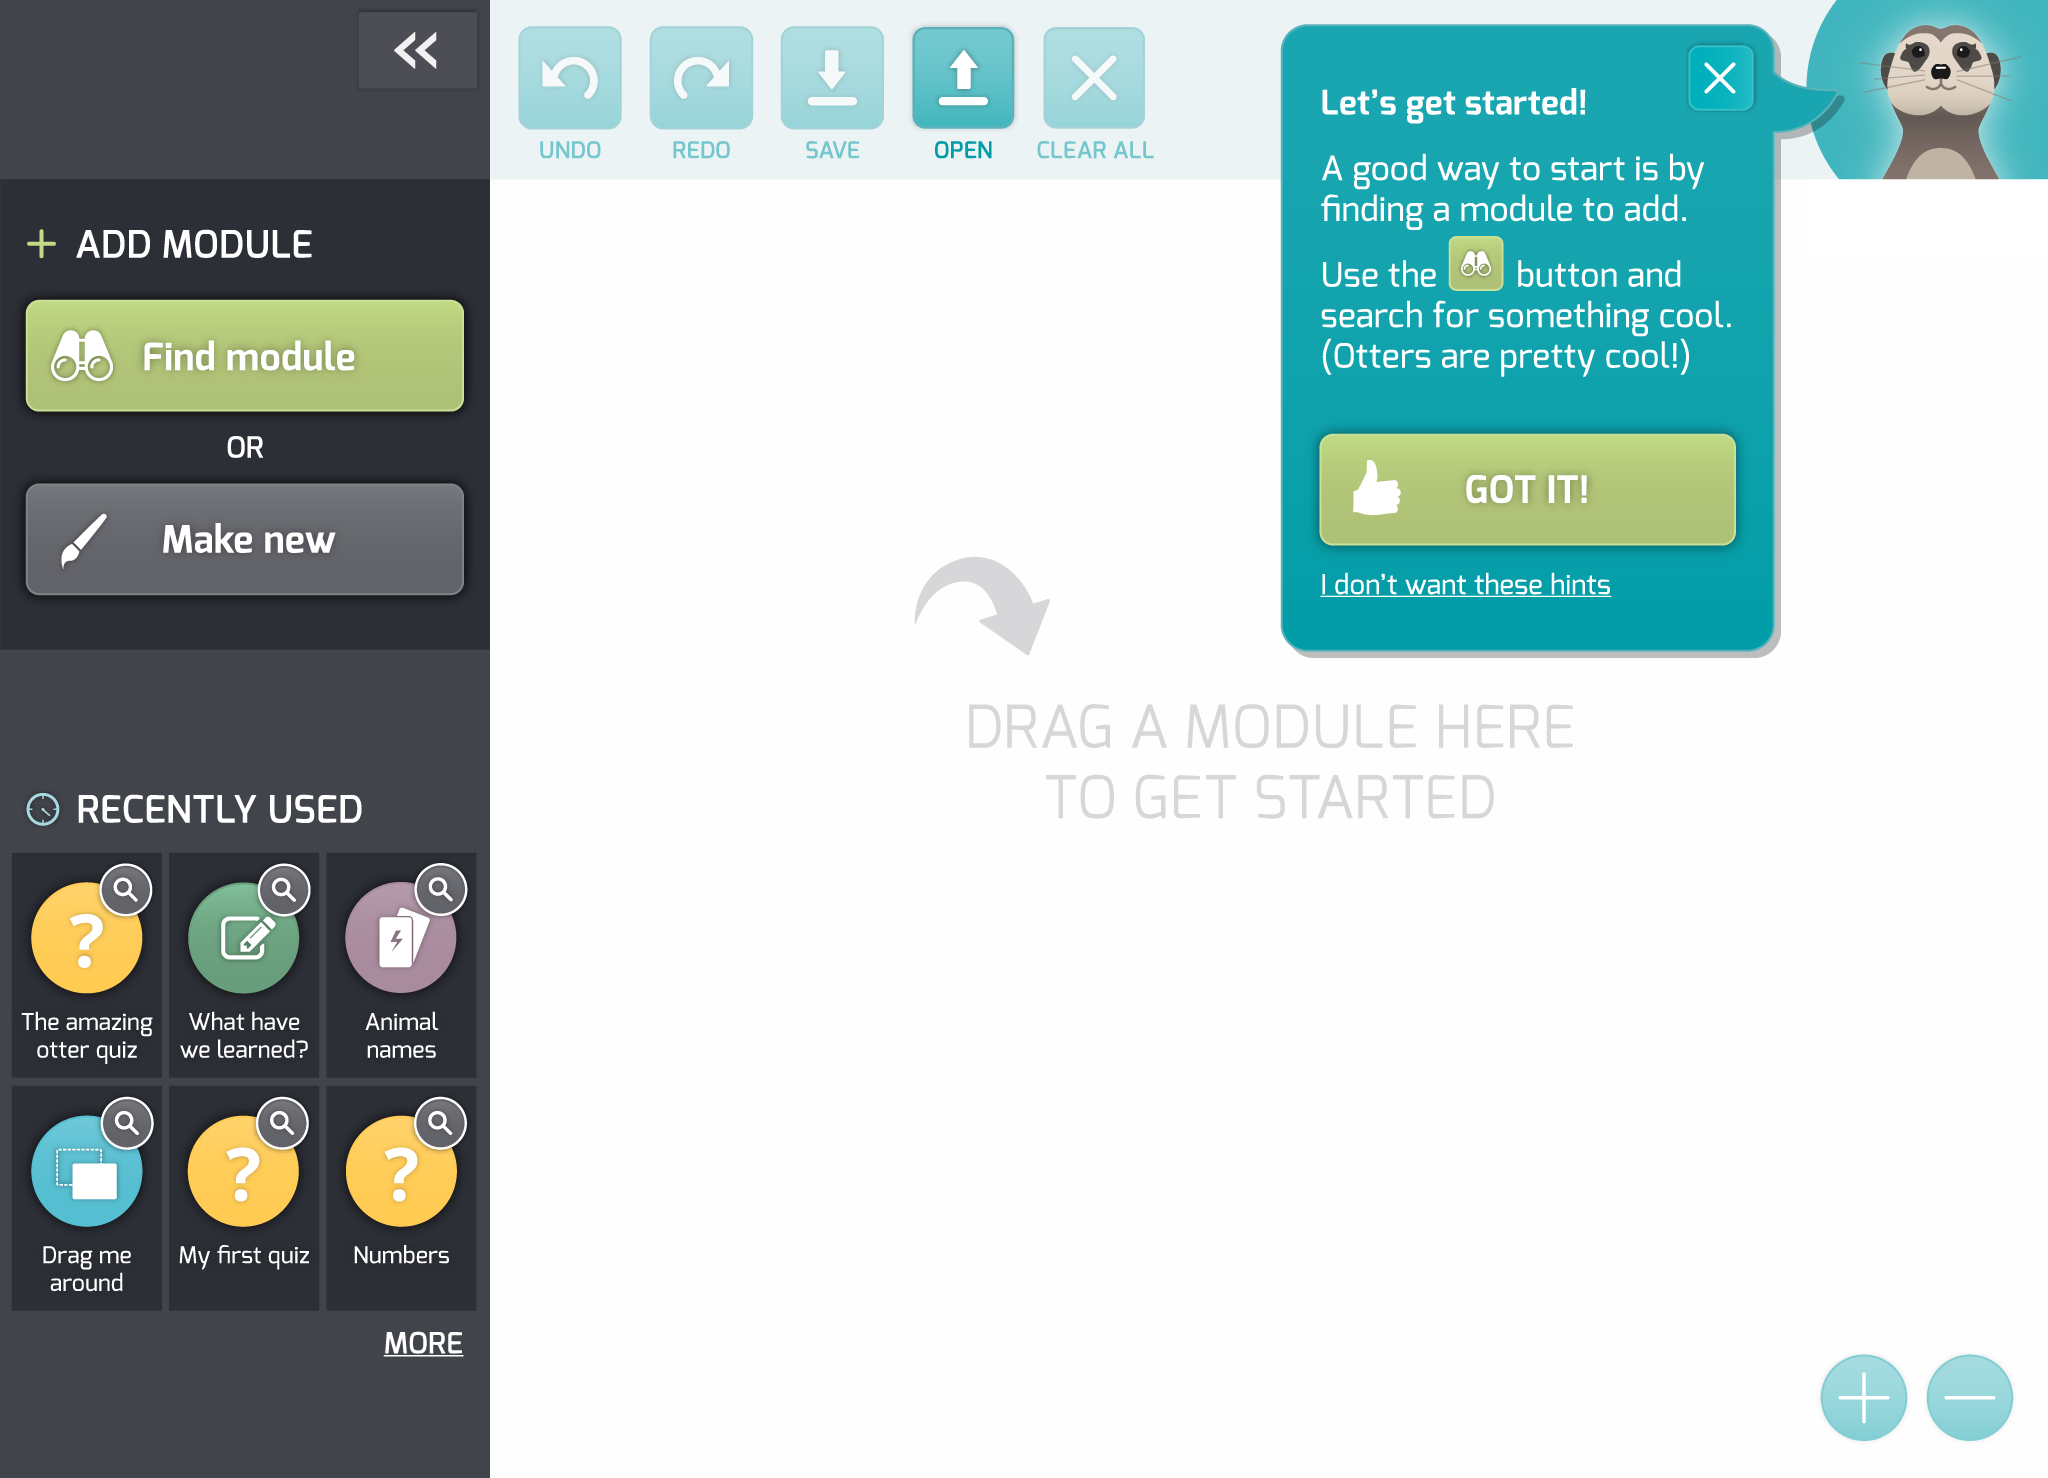
\includegraphics{fig/avatar.png}
    \end{scale}
    \caption{An avatar helping the user}
   \label{fig:avatar}
\end{figure}

Punishing bad behaviour rarely works, and punishment is easily evaded. Instead 
we simply prohibit bad behaviour. Chatting is done via the avatars. To 
communicate with another user, you visit their profile and click on their 
avatar to bring up a dial menu for constructing a query like ``you should add 
[module] to your composition!'', or ``I like this module!''. This makes 
localisation much easier since these set sentences may be translated 
accurately. It also makes our system safe for 
children\cite{sadler2012virtual}. This is a recent trend in computer games 
such as Journey and Hearthstone for the same reasons. This eliminates hate 
speech\cite{hearthstone}, which is not acceptable with a child audience.

Users may, via their avatars as just described, encourage other users by 
telling them that they like their modules. There is no way to dislike a 
module, as that might be demotivating for children. Avatars as well as modules 
may be favoured. The user's favourite modules and avatars are more easily 
accessible than the rest.

Users sign up with a log-on ID and password, and optionally an email address 
for recovering forgotten passwords. The users name their avatars which is then 
their screen names. The avatar has a name. There may be duplicate names. 
People have duplicate names in real life too [citation needed], and society 
hasn't collapsed yet. When choosing a name, feedback is given if the name is 
not unique.

\subsection{Requirements}
We place high usability requirements on our canvas system in order to enable
school children to use it.

Our target demographic at its largest is pretty much everyone that wants to 
learn or teach something. Therefore universal design is of the utmost 
importance. It is furthermore legally required in Norway\cite{uuforskrift}. 
More importantly it is The Right Thing to do. Universal design is difficult 
with such a graphical system, but of the utmost importance. Compromises shall 
err on the side of caution and favour universal design to expressiveness.

Dealing with children has interface design implications. Tap actions should 
allow some slack with bigger hit boxes than actual buttons and similar 
measurements. Splash screens are bad, mkay. Turns out kids don't have that 
great an attention-span. So get to the point quick as. These things are 
discussed in more detail in Section~\ref{principles}.

In order to encourage reuse and remixing, modules and assets are distributed 
under a free licence, CC-BY-SA\@. This also sets a positive example for school 
children to become good citizens of our society. Indeed so does the entire 
project by being licensed as AGPL\@\cite{educational}.

\subsection{Functional Details}
\subsubsection{Frontend}
For our canvas system and frontend in general we primarily use the Elm 
programming language\cite{czaplicki2012elm}.

Elm is an immature language with several known 
shortcomings\cite{smitsextreme}, but the more popular alternative JavaScript 
is a mature language with even more known 
shortcomings\cite{flanagan2006javascript}. Although early research suggests 
that using Elm will not magically result in a better 
product\cite{buist2014extending}, it does allow for purely functional 
programming of denotational graphical interfaces\cite{czaplicki2012elm}, which 
has several known advantages for interactive graphical 
programs\cite{berntsen2014quest}. Elm itself has several specific advantages 
as well --- and excellent tooling to boot\cite{kraeutmann2015functional}.

Being an immature language, not all libraries we could possibly wish for are 
readily available. Therefore accessing JavaScript directly is still useful at 
times. Thankfully, Elm comes with a sophisticated JavaScript foreign 
functional interface\cite{elmports}. And if it becomes necessary to use 
JavaScript libraries to interact with JavaScript primitives presently outside 
of Elm's reach, we may fall-back on JavaScript for this.

\subsubsection{Backend}
For dealing with all things backend we use the Haskell programming 
language\cite{marlow2010haskell}. Haskell is a mature and widely used 
programming language with advantages similar to that of Elm, except more 
advantages and more powerful advantages. Interesting advantages over Elm 
include laziness for modularisation\cite{hughes1989functional}, typeclasses 
for elegant ad-hoc polymorphism\cite{wadler1989make}, and an in general more 
powerful and interesting type system\cite{jones2003wearing}. Lastly, Haskell 
seriously equips you for all cost-models of parallelism and 
concurrency\cite{jones2012future}.

We write property laws and test these using 
QuickCheck\cite{claessen2011quickcheck}, a well-established tool used in 
industry\cite{arts2006testing}.

Haskell, being a mature language, provides us with several useful libraries to 
ensure a shorter time to market.

\subsubsection{Reuse and remix}
We want to encourage reusing and remixing. We define reuse to be using someone 
else's module as-is, and remix to be using someone else's module with 
modifications.

Care must be taken not to merely give incentives for having your modules 
reused and remixed by others, as this fosters a culture where being the author 
of novelties is the most rewarding. Rewards should therefore be doled out more 
handsomely for actually reusing and remixing than for authoring modules that 
are successfully subsequently reused and remixed. This also makes sense since 
the latter is accumulatively (having your module be reused and remixed is 
tracked and awarded recursively) rewarding passive behaviour, whilst the 
former rewards active behaviour. 

\subsection{Design document}
Given our emphasis on usability, we have had a design document authored by a 
user experience developer. This document includes a graphical profile, some 
specific user-interface design, and some overarching design principles. It may 
be found in its entirety in Appendix~\ref{design}.
